\documentclass[aspectratio=169]{beamer}

\mode<presentation> {
	\usetheme{Madrid}
	\usecolortheme{beaver}
}

\beamertemplatenavigationsymbolsempty
\definecolor{beamer@blendedblue}{rgb}{0.8,0,0}

\usepackage[czech]{babel}
\usepackage[utf8]{inputenc}
\usepackage[T1]{fontenc}
\usepackage{lmodern}
\usepackage{graphicx}
\usepackage{graphbox}
\usepackage{booktabs}
\usepackage{hyperref}

\deftranslation[to=Czech]{Example}{Příklad}

\title[Automatická kalibrace]{Systém automatické kalibrace modelového
železničního vozidla}

\author{Jan Horáček}
\institute[FI MUNI]{
	Fakulta informatiky \\
	Masarykova univerzita \\
	\medskip
	\textit{horacekj@mail.muni.cz}
}
\date{7. února 2019}

\begin{document}

%------------------------------------------------

\begin{frame}
\titlepage
\end{frame}

%------------------------------------------------

\begin{frame}
\frametitle{Cíl práce}
\begin{block}{Cíl práce}
Cílem práce je automatizovat proces kalibrace modelové lokomotivy.
\end{block}
\end{frame}

%------------------------------------------------

\begin{frame}
\frametitle{Kontext: řízení kolejiště}
\begin{figure}
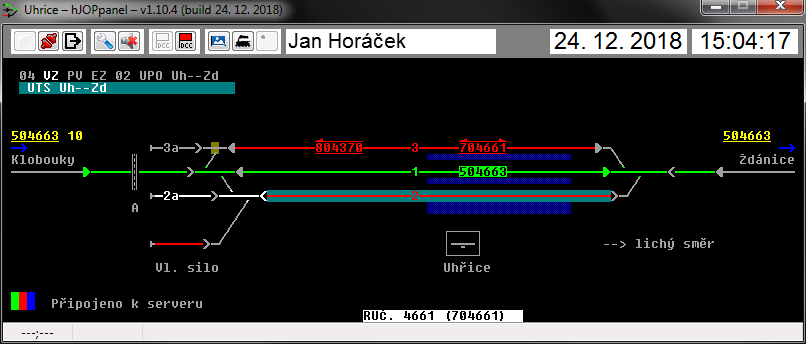
\includegraphics[width=0.7\columnwidth]{data/hJOPpanel-uh.png}
\end{figure}
\end{frame}

%------------------------------------------------

\begin{frame}
\frametitle{Kontext: řízení kolejiště}
\begin{figure}
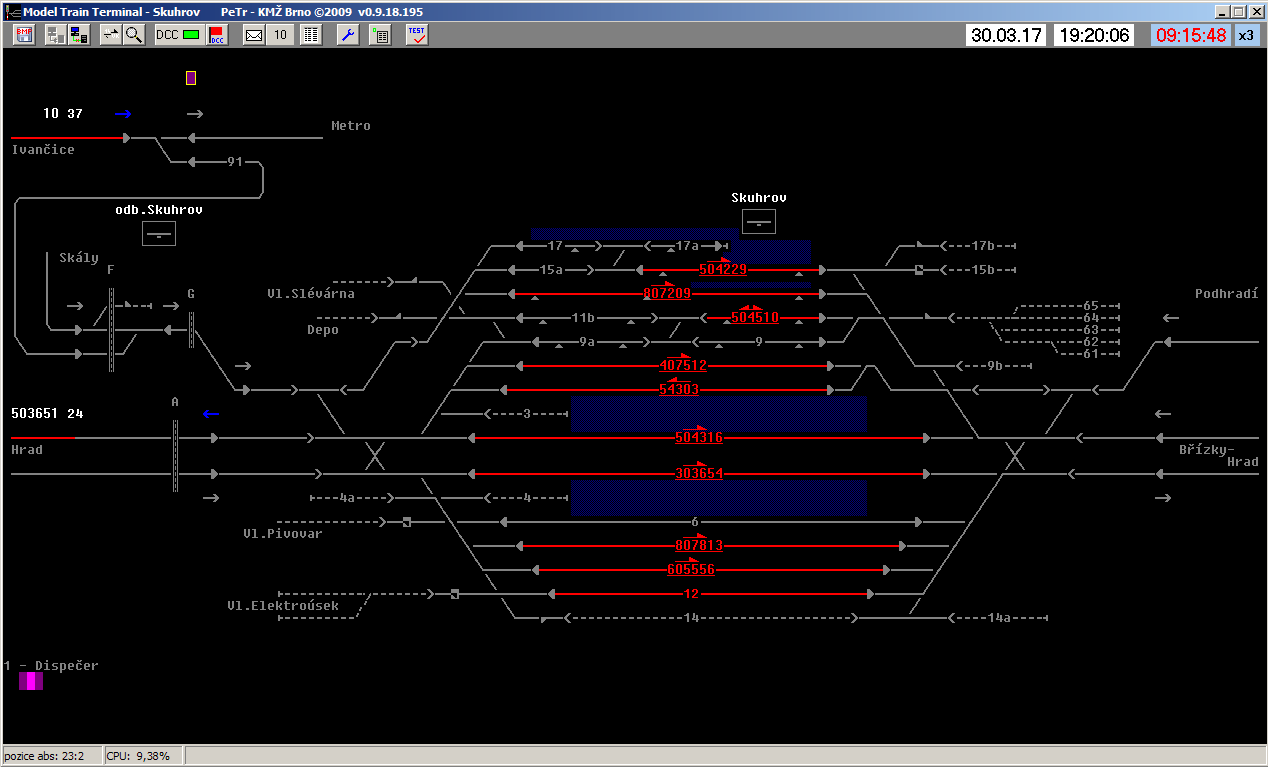
\includegraphics[width=0.75\columnwidth]{data/JOP2-SkLogin.png}
\end{figure}
\end{frame}

%------------------------------------------------

\begin{frame}
\frametitle{Kontext: digitální řízení vlaku}
Digital Command Control (DCC):
\begin{itemize}
\item Každá lokomotiva obsahuje miniaturní počítač, tzv. \uv{dekodér}.
\item DCC centrála generuje data pro lokomotivy.
\item Lokomotiva data přijímá a na základě nich koná akce.
\item Každá lokomotiva má svou číselnou adresu, kterou je identifikována (typicky
$1$--$9999$).
\item Centrála generuje DCC signál na základě povelů z~ovladačů.
\begin{itemize}
\item ruční ovladač, počítač, ...
\end{itemize}
\item Dekodér je možno konfigurovat: ukládat do něj číselné hodnoty do jednotlivých
konfiguračních slotů (tzv. \textit{CV}).
\end{itemize}

TODO obrázek topologie kolejiště
\end{frame}

%------------------------------------------------

\begin{frame}
\frametitle{Kontext: řízení kolejiště počítačem}
\begin{itemize}
\item Jízdu vlaku řídí počítač, obsluha vydává povely typu: \uv{Vlaku 8013, jeď
na třetí kolej do vedlejší stanice!}.
\item Správce systému volí, jak rychle se mají kde vlaky pohybovat (km/h).
\item Rychlost lokomotivy z pohledu dekodéru = číslo $0$--$28$ a směr $0$/$1$.
\end{itemize}
$\Rightarrow$ Nutnost spárovat skutečnou rychlost a jízdní stupeň.
\end{frame}

%------------------------------------------------

\begin{frame}
\frametitle{Kalibrace}
\begin{block}{Kalibrace}
\begin{enumerate}
\item Nakonfigurování dekodéru tak, aby konkrétnímu jízdnímu stupni odpovídala
konkrétní skutečná rychlost.
\item Nakonfigurování dekodéru tak, aby z~rychlosti $40$~km/h mělo hnací vozidlo
brzdnou dráhu $30$--$35$~cm.
\end{enumerate}
\end{block}

\pause

\begin{block}{Vybrané přínosy}
\begin{itemize}
\item Zastavení vlaku na správném místě.
\item Očekávatelné prostředí pro obsluhu.
\item Přípřeže, postrky.
\end{itemize}
\end{block}

Současná kalibrace je ruční $\Rightarrow$ automatizovat.
\end{frame}

%------------------------------------------------

\begin{frame}
\frametitle{Automatická kalibrace}
\begin{enumerate}
\item Nástroj pro měření rychlosti: měřicí vůz.
\item Počítačový program.
\end{enumerate}
\end{frame}

%------------------------------------------------

\begin{frame}
\frametitle{Měřicí vůz}
\begin{columns}[t]
	\column{.5\textwidth}
	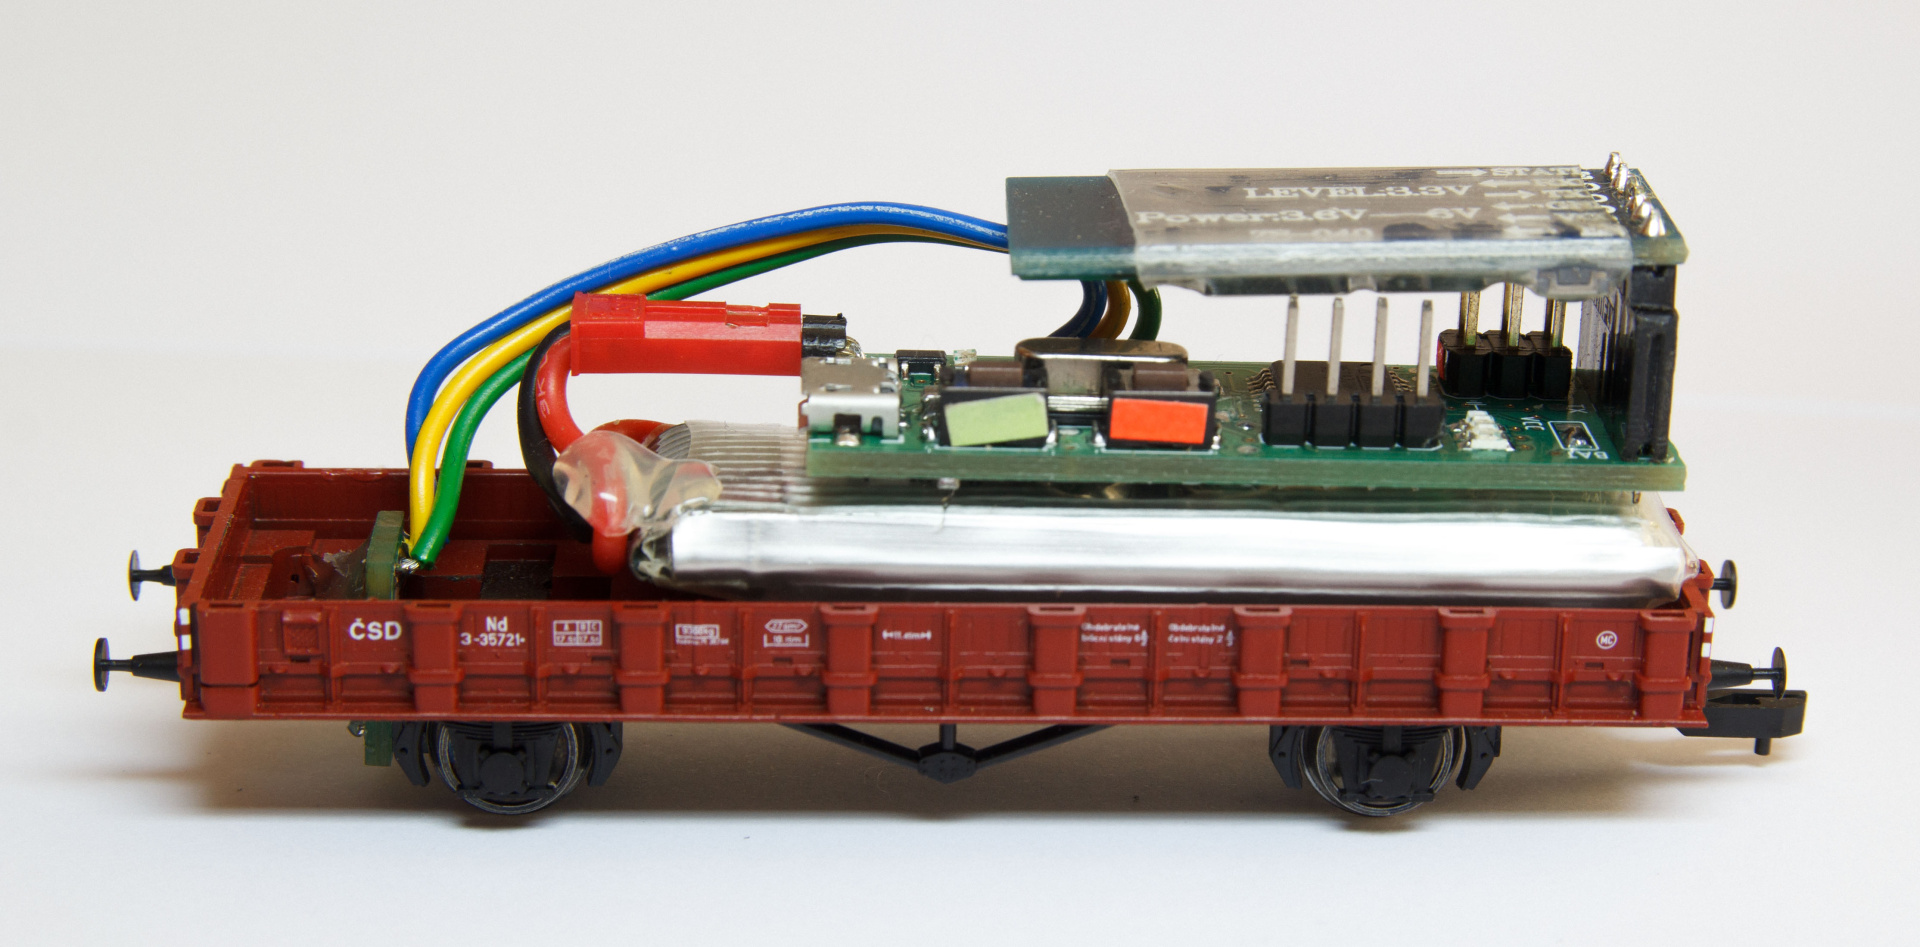
\includegraphics[width=\columnwidth]{data/wsm-3d.jpg}
	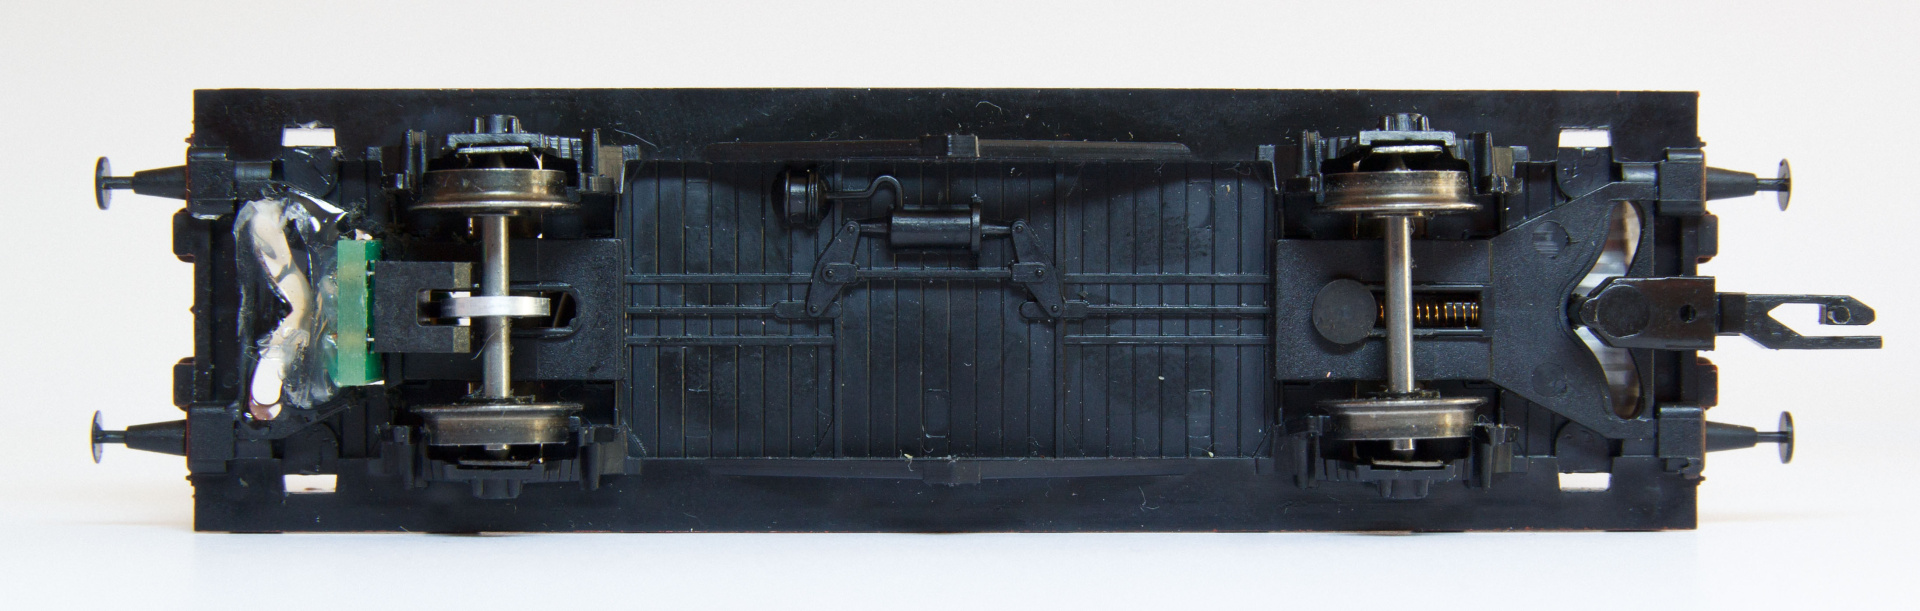
\includegraphics[width=\columnwidth]{data/wsm-bot.jpg}
	\column{.5\textwidth}
	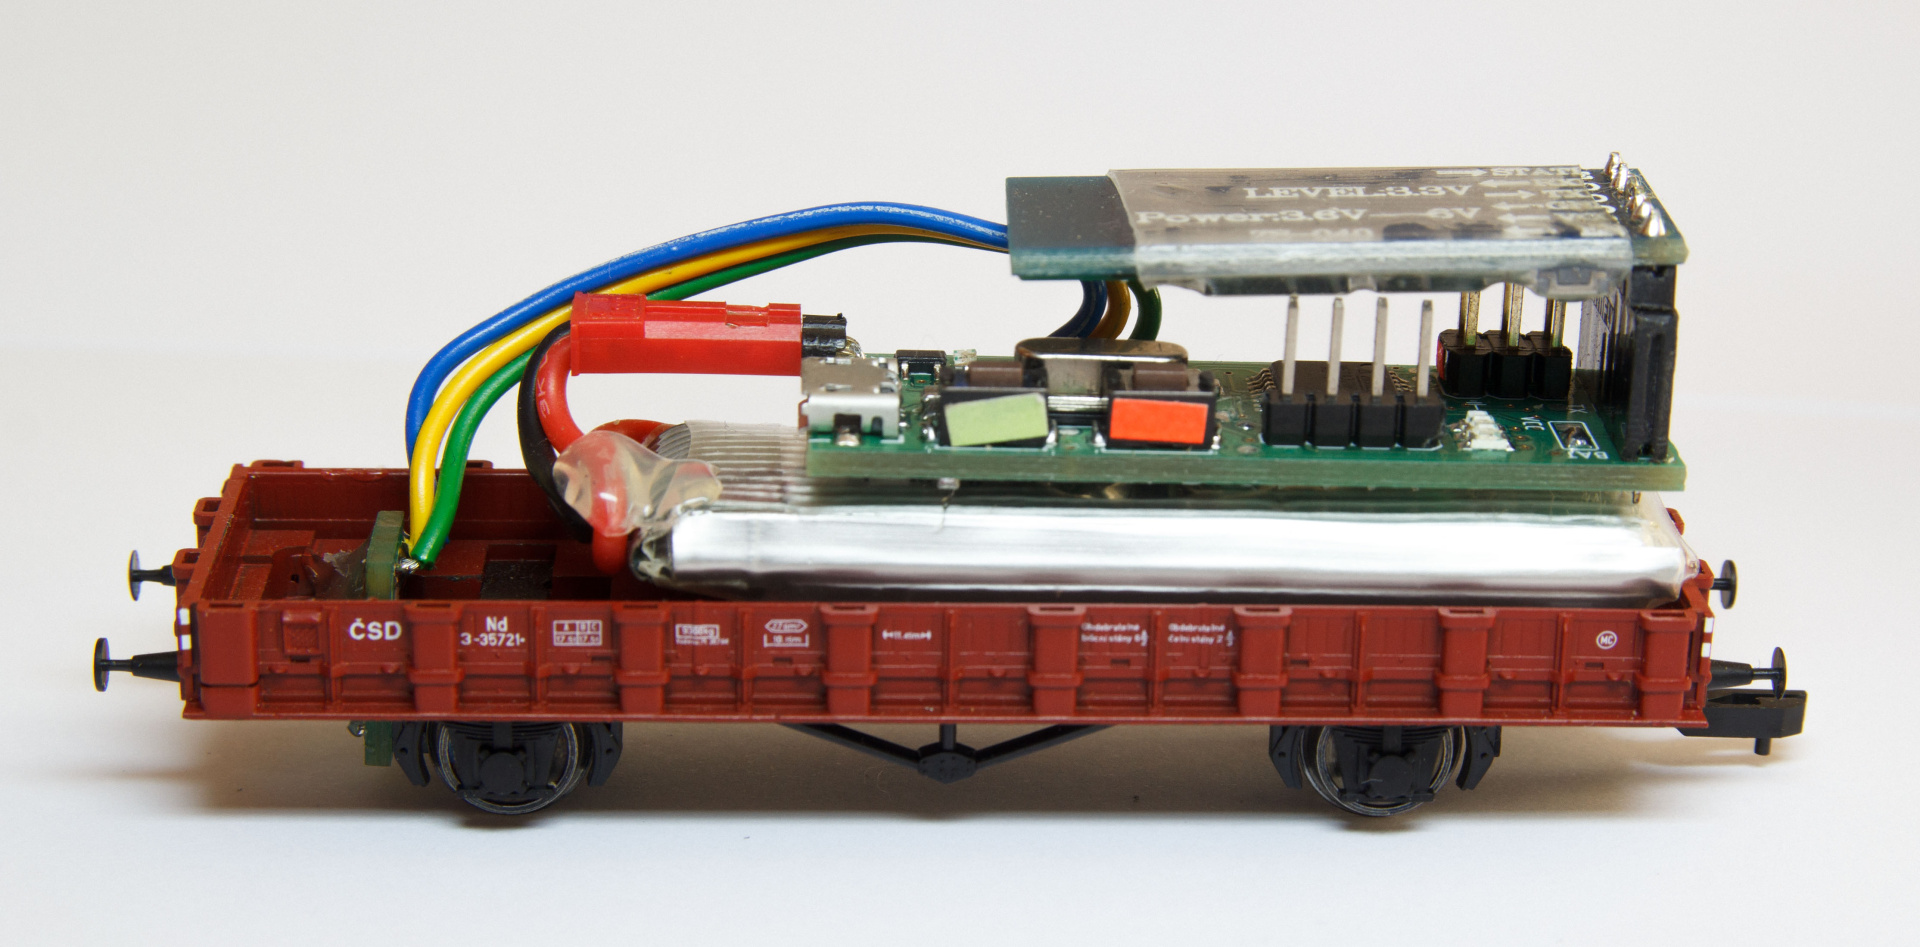
\includegraphics[width=\columnwidth]{data/wsm-3d.jpg}
	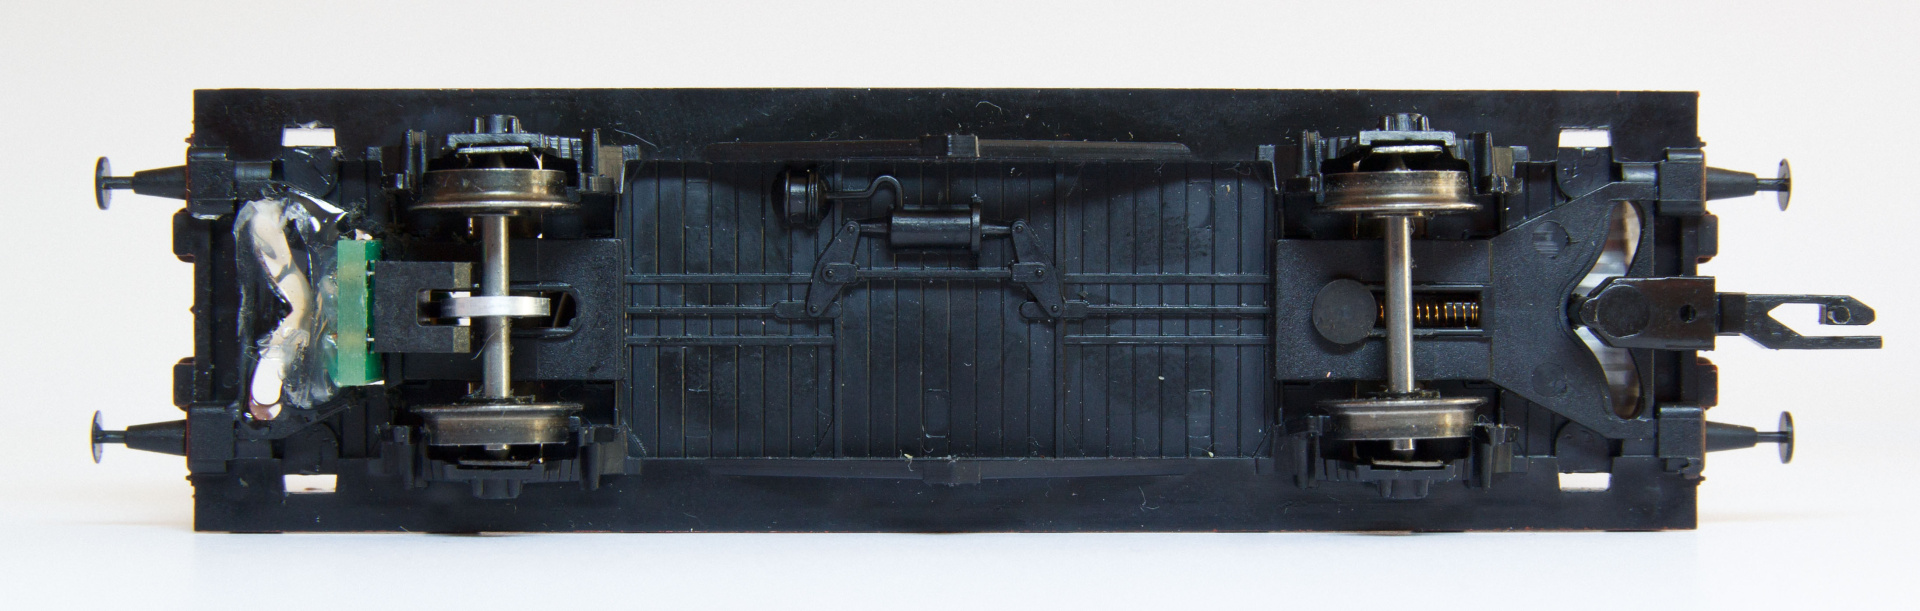
\includegraphics[width=\columnwidth]{data/wsm-bot.jpg}
\end{columns}
\end{frame}

%------------------------------------------------

\begin{frame}
\frametitle{Software}
\begin{columns}[t]
	\column{.35\textwidth}
	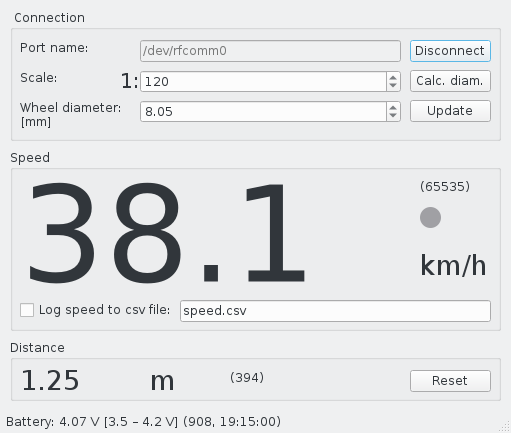
\includegraphics[align=c,width=\columnwidth]{data/speed_reader_screenshot.png}
	\pause
	\column{.65\textwidth}
	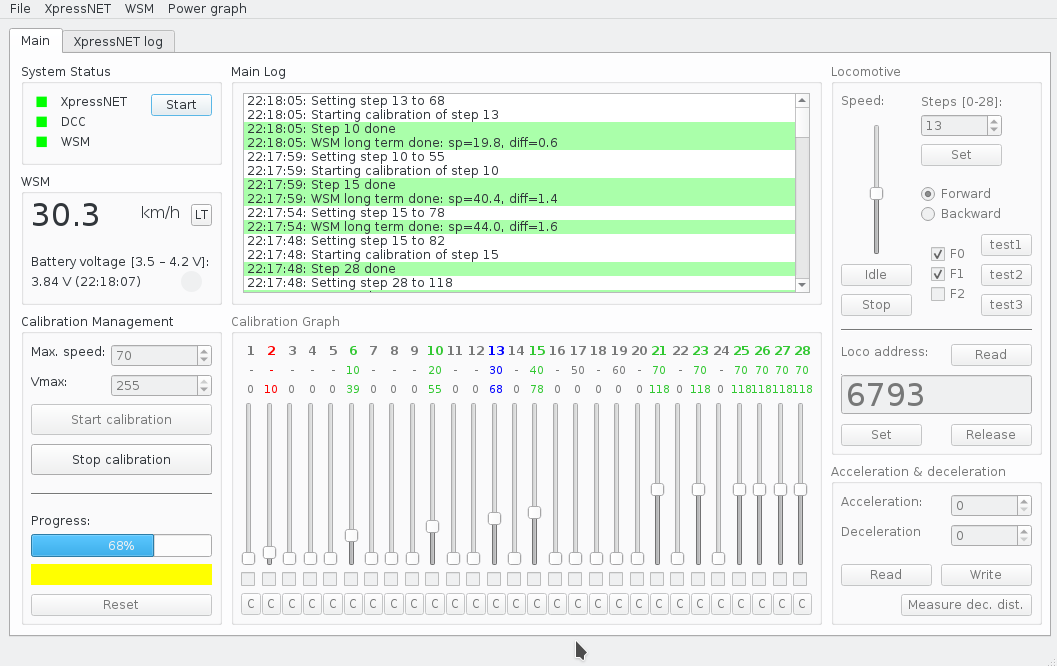
\includegraphics[align=c,width=\columnwidth]{data/ac_progress.png}
\end{columns}
\end{frame}

%------------------------------------------------

\begin{frame}
\frametitle{Ukázka}
Video
\end{frame}

%------------------------------------------------

\begin{frame}
\frametitle{Přínos}
\begin{itemize}
\item Fungující proof-of-concept.
\item Kalibrace: 25 minut + člověk $\rightarrow$ 4 minuty autonomně.
\item Autor si prošel realizací své vize od prvotního nápadu až po finální produkt.
\item Univerzální měřicí vůz.
\item Zajímavá naměřená data.
\item Vytvořena spousta zajímavého opensource SW (XpressNET knihovna).
\end{itemize}
\end{frame}

%------------------------------------------------

\end{document}
